%!TEX root = main.tex
\section{Evaluation}
\label{sec:evaluation}
\subsection{Experimental setup}
\textbf{Server.}
The experiments were conducted on a server equipped with
8 NVIDIA Tesla A100 GPUs (40 GB each) connected via PCIe 4.0 ×16,
an AMD EPYC 7402 2.8 GHz 24-core processor, and 504 GB of memory.
The server runs CentOS 7 and is configured with the CUDA Toolkit 11.2, cuDNN 8.4.1, PyTorch 1.11,
and Huggingface Transformers~\cite{wolf2020transformers} version 4.27.2. The NCCL library version used is 2.10.3.

\textbf{Workloads.} We evaluate our approach using four state-of-the-art deep learning models:
BERT~\cite{devlinBERTPretrainingDeep2019}, GPT-2~\cite{radfordLanguageModelsAre2019},
T5 (Text-to-Text Transfer Transformer)~\cite{raffelExploringLimitsTransfer2020}, and AmoebaNet~\cite{realRegularizedEvolutionImage2019}.
BERT, developed by Google AI Language, has 1024 hidden layers and approximately 340 million parameters.
GPT-2, a well-known pre-trained model by OpenAI, has shown significant success across various NLP tasks.
For our evaluation, we use the large version with around 770 million parameters.
T5, a sequence-to-sequence model from Google,
is tested in its large version containing approximately 780 million parameters.
AmoebaNet, a neural network generated using the Neural Architecture Search (NAS) algorithm, has about 28 million parameters.
BERT and GPT-2 are trained on the WikiText-103~\cite{merityPointerSentinelMixture2017} dataset,
while T5 is trained on the WMT-16~\cite{bojarFindings2016Conference2016} dataset, with all three models using the Adam optimizer.
AmoebaNet is trained on the ImageNet~\cite{dengImagenetLargeScaleHierarchical2009}
dataset with the stochastic gradient descent (SGD) optimizer.
We evaluate two pipeline configurations with 4 and 8 stages.

\textbf{Baselines.}
We have set up four baselines to evaluate the memory efficiency and training performance, which are listed below.
\begin{itemize}
  \item ZeRO~\cite{rajbhandariZeROMemoryOptimizations2020}: ZeRO is developed by Microsoft
  to eliminate redundant parameter storage across GPUs in data parallel training.
  We include optimization levels ZeRO-2 and ZeRO-3 in our evaluation.
  \item GPipe~\cite{huangGpipeEfficientTraining2019}: GPipe is originally implemented based on Lingvo~\cite{shen2019lingvo}
   we instead use torchgpipe~\cite{kimTorchgpipeOntheflyPipeline2020}, a PyTorch reimplementation of GPipe, for our evaluation.
  \item PipeDream~\cite{narayananPipeDreamGeneralizedPipeline2019}: PipeDream profiles the model at runtime
  and uses dynamic programming to minimize the longest computation time across all stages.
  \item vPipe~\cite{zhaoVPipeVirtualizedAcceleration2022}: vPipe is built on PipeDream’s runtime
  while its partitioning algorithm is not open-sourced.
  Therefore, we implemented it according to the description provided in the corresponding paper of vPipe.
\end{itemize}

\subsection{Memory Using Efficiency}
In this section, we assess the maximum trainable batch size
for each method to evaluate GPU memory efficiency.
The batch size is determined by multiplying the micro-batch size
by the number of splits in synchronous pipeline parallelism.
We compare micro-batch sizes in asynchronous pipeline parallel training,
as it differs from synchronous training,
where there is a distinct gap between the computations of consecutive batches.

\subsubsection{Synchronous Pipeline Parallel Training}
We first evaluate the synchronous pipeline parallel training mode.
In this experiment, the number of micro-batches is equal to the number of pipeline stages.
The results are shown in Table~\ref{table:maxbs-sync},
where the synchronous training modes of vPipe and DawnPiper are denoted as vPipe-S and DPiper-S, respectively.

The results indicate that ZeRO-2 and ZeRO-3 achieve nearly the same maximum batch sizes across the four models.
In fact, the maximum batch sizes of ZeRO-3 are even smaller for the T5 and AmoebaNet models.
This is because, as the batch size increases, the additional memory saved
by ZeRO-3's model parameter optimizations is no longer sufficient to support larger batches,
as ZeRO-3 also requires extra memory buffers for communication.
For GPipe and vPipe, the maximum batch sizes are generally comparable to ZeRO for BERT, GPT-2, and T5.
However, they are significantly smaller than ZeRO for the AmoebaNet model.
This difference arises because in Transformer-based models,
the computation and memory usage of each layer are roughly proportional.
As a result, GPipe and vPipe, which aim to balance computation time across stages,
can also effectively balance memory usage.
In contrast, CNN models like AmoebaNet have layers where computation time and memory usage are often not proportional.
For instance, a convolutional layer may have a long computation time but minimal memory usage,
leading to an uneven memory footprint when balancing computation time across stages.
Consequently, the maximum batch sizes that GPipe and vPipe achieve on AmoebaNet
are only 68\% and 46\% of those achieved by ZeRO when the number of pipeline stages is 4.
These ratios drop further to 58\% and 32\% as the number of pipeline stages increases to 8.
Meanwhile, GPipe supports larger batch sizes than vPipe,
but the result reverses when memory optimization is enabled.
This reversal occurs because the stage with the memory bottleneck shifts when memory optimization is applied.

DawnPiper achieves the largest batch sizes among all methods for the BERT, GPT-2, and T5 models.
Without memory optimization, it increases the batch size by up to 1.2$\times$ and 1.55$\times$
compared to the second-best method, vPipe, when the pipeline stages are 4 and 8, respectively.
Note that for GPT-2,
the maximum batch sizes remain consistent across all methods
due to the model's substantial memory footprint during training,
where even a slight increase in batch size results in a significant rise in memory usage.
Although DawnPiper refines the pipeline partitioning,
it cannot further increase the batch size under these conditions.
For AmoebaNet, DawnPiper's maximum batch size is slightly smaller than ZeRO’s,
as data parallelism can more effectively divide the memory footprint across GPUs,
which is challenging for pipeline parallelism.
Nonetheless, DawnPiper outperforms GPipe and vPipe with batch size increases of 1.29$\times$ and 1.91$\times$
when the pipeline stages are set to 4.
As the number of stages increases to 8, it still surpasses GPipe and vPipe by up to 1.17$\times$ and 2.12$\times$, respectively.

With memory optimization enabled, DawnPiper continues to achieve the largest batch sizes.
Compared to the second-best method, vPipe, DawnPiper increases the maximum batch size by
an average of 1.33$\times$ and 1.29$\times$ for pipeline stages of 4 and 8, respectively.
Additionally, the results show that the average batch size achieved by DawnPiper
increases by 1.84$\times$ as the number of pipeline stages doubles, demonstrating its strong memory scalability.
\begin{table}[htbp]
  \centering
  \caption{Maximum Batch Size in Synchronous Pipeline Parallelism}
    \begin{tabular}{m{2em}|m{2em}|ccccc}
    \toprule
    \#\ GPU & MO & Method & BERT & GPT-2 & T5 & AmoebaNet \\
    \midrule
    \multirow{8}{*}{4} & \multirow{5}{*}{None} & ZeRO-2 & 64    & 8     & 140   & 412 \\
          &       & ZeRO-3 & 64    & 8     & 132   & 404 \\
          &       & GPipe & 52    & 8     & 144   & 280 \\
          &       & vPipe-S & 60    & 8     & 144   & 188 \\
          &       & \textbf{DPiper-S} & \textbf{72} & \textbf{8} & \textbf{160} & \textbf{360} \\
\cmidrule{2-7}          & R & GPipe & 120   & 28    & 348   & 644 \\
\cmidrule{2-2}          & \multirow{2}{*}{S+R} & vPipe-S & 128   & 28    & 348   & 720 \\
          &       & \textbf{DPiper-S} & \textbf{160} & \textbf{32} & \textbf{424} & \textbf{1220} \\
    \midrule
    \multirow{8}{*}{8} & \multirow{5}{*}{None} & ZeRO-2 & 128   & 16    & 224   & 824 \\
          &       & ZeRO-3 & 128   & 16    & 208   & 808 \\
          &       & GPipe & 88    & 16    & 256   & 480 \\
          &       & vPipe-S & 88    & 16    & 256   & 264 \\
          &       & \textbf{DPiper-S} & \textbf{136} & \textbf{16} & \textbf{320} & \textbf{560} \\
\cmidrule{2-7}          & R & GPipe & 208   & 48    & 664   & 1384 \\
\cmidrule{2-2}          & \multirow{2}{*}{S+R} & vPipe-S & 208   & 56    & 664   & 1424 \\
          &       & \textbf{DPiper-S} & \textbf{280} & \textbf{60} & \textbf{800} & \textbf{2180} \\
    \bottomrule
    \end{tabular}%
  \label{table:maxbs-sync}%
\end{table}

% Table generated by Excel2LaTeX from sheet '工作簿2'
\begin{table}[htbp]
  \centering
  \caption{Maximum Batch Size in ASynchronous Pipeline Parallelism}
    \begin{tabular}{m{2em}|m{2em}|m{5em}cccc}
    \toprule
    \#\ GPU & MO & Method & BERT & GPT-2 & T5 & AmoebaNet \\
    \midrule
    \multirow{5}{*}{4} & \multirow{3}{*}{None} & PipeDream & 16    & 2     & 40    & 70 \\
          &       & vPipe-AS & 16    & 2     & 40    & 48 \\
          &       & \textbf{DPiper-AS} & \textbf{32} & \textbf{3} & \textbf{78} & \textbf{150} \\
\cmidrule{2-7}          & \multirow{2}{*}{S+R} & vPipe-AS & 46    & 8     & 110   & 300 \\
          &       & \textbf{DPiper-AS} & \textbf{84} & \textbf{10} & \textbf{192} & \textbf{480} \\
    \midrule
    \multirow{5}{*}{8} & \multirow{3}{*}{None} & PipeDream & 16    & 2     & 44    & 64 \\
          &       & vPipe-AS & 16    & 2     & 44    & 32 \\
          &       & \textbf{DPiper-AS} & \textbf{40} & \textbf{5} & \textbf{84} & \textbf{128} \\
\cmidrule{2-7}          & \multirow{2}{*}{S+R} & vPipe-AS & 58    & 16    & 144   & 214 \\
          &       & \textbf{DPiper-AS} & \textbf{100} & \textbf{22} & \textbf{248} & \textbf{528} \\
    \bottomrule
    \end{tabular}%
  \label{table:maxbs-async}%
\end{table}

\subsubsection{ASynchronous Pipeline Parallel Training}
In this section, we evaluate memory efficiency in the asynchronous pipeline parallel training mode.
The results are shown in Table ~\ref{table:maxbs-async},
where the asynchronous modes of vPipe and DawnPiper are denoted as vPipe-AS and DPiper-AS, respectively.

With memory optimization disabled,
DawnPiper significantly increases the maximum batch size compared to PipeDream and vPipe,
as GPU memory usage is more unbalanced in asynchronous pipeline parallel training.
Across the four models,
DawnPiper increases the maximum batch size by an average of 2.14$\times$ and 2.73$\times$ compared to vPipe
when the pipeline stages are 4 and 8, respectively.
Compared to PipeDream, the improvement ranges from 4.8$\times$ to 11$\times$.
This improvement is due to DawnPiper’s ability to refine
pipeline partitioning and fully utilize available GPU memory resources.
For AmoebaNet specifically, the increases are 3.13$\times$ and 4$\times$, respectively,
as vPipe is primarily designed for Transformer-based models and does not support CNN models effectively.
With memory optimization enabled, DawnPiper still achieves a 1.61$\times$ and 1.82$\times$
increase in maximum batch size compared to vPipe when the pipeline stages are 4 and 8, respectively.

\subsection{Training Performance}
In this section, we evaluate the training speed of each method under the same batch size.
Since batch size in asynchronous pipeline parallel frameworks is not well-defined,
we use the micro-batch size for performance comparisons.
Note that ZeRO and PipeDream can only operate with small micro-batch sizes before encountering memory oversubscription,
so they are excluded from this comparison.
Nonetheless, we can still gain a general understanding of their performance.
For instance, ZeRO achieves 1.4$\times$ the training speed of GPipe
on the relatively small BERT model at a smaller batch size,
but its speed drops to just 20\% of GPipe's on the larger GPT-2 model.
As for PipeDream, its performance is similar to vPipe,
with the main distinction being a more noticeable difference in model partitioning on AmoebaNet,
while differences in other cases are relatively minor.
\begin{figure}[tb]
  \centering
  % \hspace{-0.7cm}
  \subfigure[BERT]{
    \centering
    \label{subfig:bert-4}
    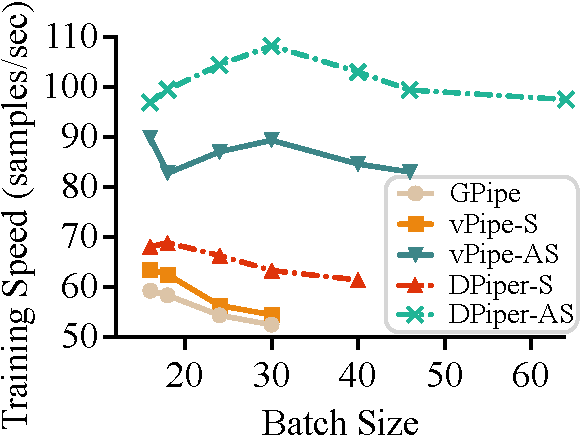
\includegraphics[width=0.47\linewidth]{BERT-4GPU-crop.pdf}
  }
  \subfigure[GPT-2]{
    \centering
    \label{subfig:gpt-2-4}
    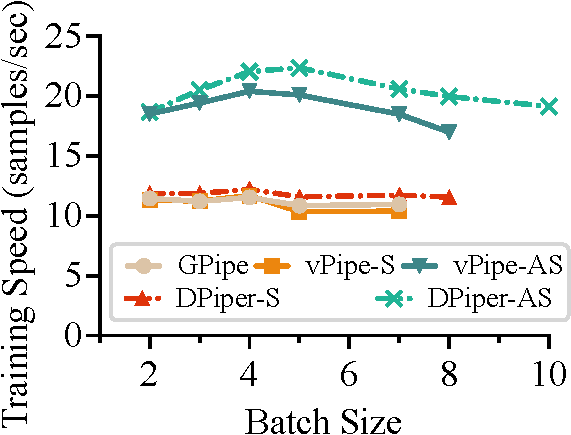
\includegraphics[width=0.47\linewidth]{GPT-2-4GPU-crop.pdf}
  }
  \subfigure[T5]{
    \centering
    \label{subfig:t5-4}
    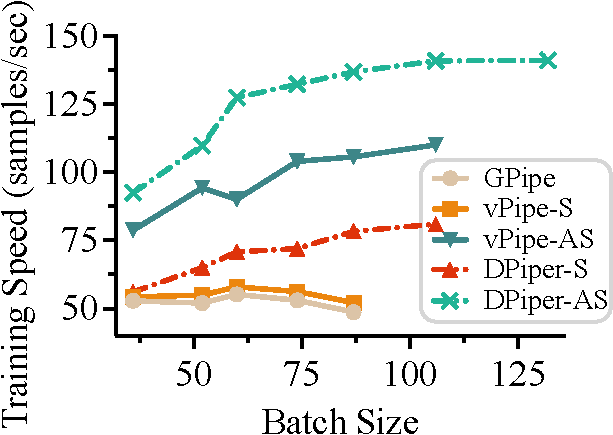
\includegraphics[width=0.47\linewidth]{T5-4GPU-crop.pdf}
  }
  \subfigure[AmoebaNet]{
    \centering
    \label{subfig:amoebanet-4}
    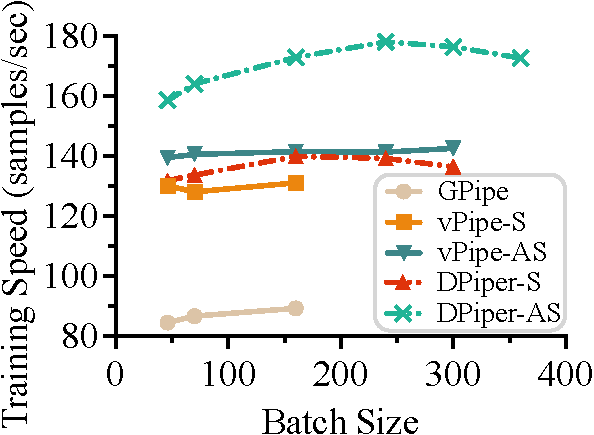
\includegraphics[width=0.47\linewidth]{AmoebaNet-4GPU-crop.pdf}
  }
  \caption{Training Speed under Pipeline Stage of 4}
  \label{fig:perf-4}
\end{figure}

The training speed comparison for a pipeline stage of 4 is shown in Figure~\ref{fig:perf-4}.
The performance of synchronous pipeline parallelism is significantly
lower than that of asynchronous pipeline parallelism due to pipeline bubbles caused by computation synchronization.
Overall, vPipe-S outperforms GPipe, with a more noticeable advantage on AmoebaNet.
This is because GPipe does not account for communication overhead between stages,
leading to inefficient partitions in CNN models and higher communication volumes.
In contrast, both DawnPiper and vPipe take communication overhead into account when determining pipeline partitioning.

At smaller batch sizes, DawnPiper does not exhibit a significant advantage over other methods,
with an average performance improvement of around 7\%,
and only a 17\% and 14\% improvement in asynchronous training on the T5 and AmoebaNet models, respectively.
This is because, when memory is not oversubscribed,
DawnPiper’s main benefit comes from refining the pipeline partition to find a better model split.

As the batch size increases, other methods must implement memory optimization to meet the training requirements.
At this point, DawnPiper shows a clear increase in training speed compared to the others.
This improvement stems from two factors. Firstly, GPU resources are better utilized as the batch size grows.
Secondly, DawnPiper can: (a) adjust the memory footprint of each stage with minimal impact on computation time,
and (b) reduce the memory footprint with negligible performance overhead using memory swapping for relatively small batch sizes.
The first advantage is possible due to insights on memory usage during training, as discussed in Section~\ref{sec:mot}.
Consequently, in synchronous pipeline parallelism,
DawnPiper achieves up to a 1.5$\times$ performance improvement on T5 as the batch size increases
and up to a 1.41$\times$ improvement in asynchronous mode.
Overall, as the batch size grows,
DawnPiper delivers an average performance improvement of 1.2$\times$, 1.12$\times$, 1.32$\times$, and 1.24$\times$ over vPipe
in asynchronous parallel training on BERT, GPT-2, T5, and AmoebaNet, respectively.
\begin{figure}
  \centering
  % \hspace{-0.7cm}
  \subfigure[GPT-2]{
    \centering
    \label{subfig:gpt-2-8}
    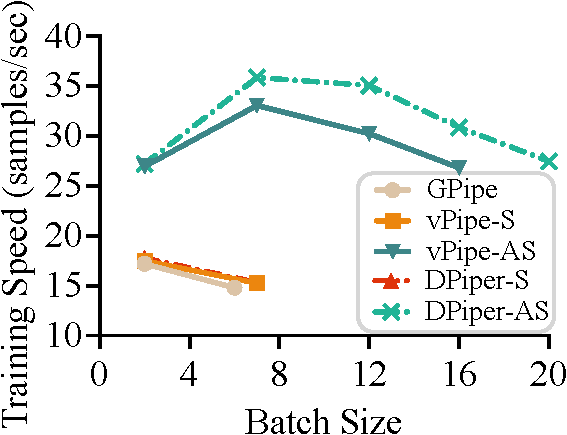
\includegraphics[width=0.47\linewidth]{GPT-2-8GPU-crop.pdf}
  }
  \subfigure[T5]{
    \centering
    \label{subfig:t5-8}
    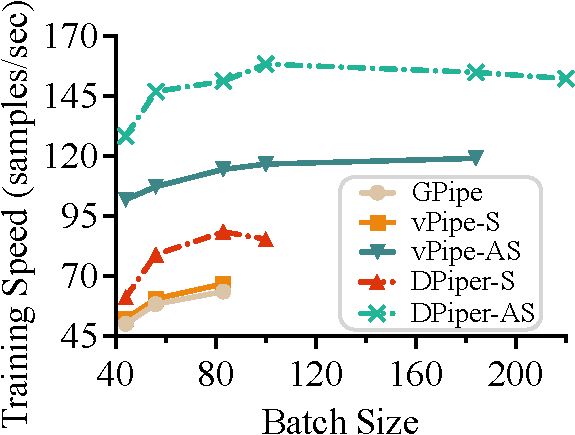
\includegraphics[width=0.47\linewidth]{T5-8GPU-crop.pdf}
  }
  \caption{Training Speed under Pipeline Stage of 8}
  \label{fig:perf-8}
\end{figure}

Evaluations were conducted only on GPT-2 and T5 when the number of pipeline stages increased to 8,
as the model sizes of BERT and AmoebaNet are too small to fully utilize 8 GPUs.
The results are presented in Figure~\ref{fig:perf-8}.
In synchronous mode, the performance of GPT-2 on DawnPiper, GPipe, and vPipe is comparable.
This similarity arises because the optimal partition points for computation and memory in GPT-2 are closely aligned,
limiting the space for partition optimization.
In asynchronous mode, as the batch size gradually increases,
DawnPiper's training speed is on average 1.15$\times$ faster than vPipe on GPT-2 and 1.34$\times$ faster on T5.
DawnPiper shows greater performance improvement on T5 due to its mixed architecture,
which combines both encoder and decoder,
offering a more complex structure that provides greater partitioning opportunities.
Furthermore, as the number of pipeline stages increases to 8, DawnPiper demonstrates strong scalability.

\subsection{Detailed analysis on computation time and memory footprint}
To provide a more detailed comparison of the memory footprint and computation performance between DawnPiper and vPipe,
we profiled the GPU peak memory usage and computation time of each stage on T5 in asynchronous mode with 8 pipeline stages.
The micro-batch size was set to 110, which is 2.5$\times$ larger
than the maximum batch size vPipe can handle without memory optimization.
The results are presented in Figure~\ref{fig:mem-comp}.

Regarding peak memory usage per stage, DawnPiper uses more GPU memory than vPipe,
but with more balanced memory distribution across stages.
This is because vPipe applies a coarser-grained pipeline partitioning and memory optimization,
whereas DawnPiper implements finer-grained memory optimizations tailored to each stage’s requirements.
As a result, overall GPU memory utilization is improved by 17.8\% compared to vPipe.
Additionally, DawnPiper’s partition strategy leads to more balanced computation times across stages,
with the difference between the longest and shortest stage execution times being only 7.7\%,
compared to 35.8\% under vPipe’s partition and memory optimization strategy.
\begin{figure}
  \centering
  \includegraphics*[width=0.8\linewidth]{mem-comp.pdf}
  \caption{Peak Memory Usage and Computation time Analysis}
  \label{fig:mem-comp}
\end{figure}
